\documentclass[11pt]{article}

\usepackage{acl}
\usepackage{times}
\usepackage{latexsym}
\usepackage[T1]{fontenc}
\usepackage[utf8]{inputenc}
\usepackage{microtype}
\usepackage{graphicx}
\usepackage{amsmath}
\usepackage{amssymb}
\usepackage{booktabs}
\usepackage{multirow}
\usepackage{xcolor}
\usepackage{tikz}
\usetikzlibrary{arrows.meta,positioning,fit,calc}

\newcommand{\method}{CA-EasyRec}
\newcommand{\base}{EasyRec}
\newcommand{\pending}{\textemdash}
\definecolor{lightblue}{RGB}{232,242,252}
\definecolor{lightgreen}{RGB}{232,247,239}
\definecolor{lightorange}{RGB}{253,241,226}

\title{Confidence-Aware EasyRec: Mitigating False Negatives in\\
Contrastive Language Modeling for Personalized Recommendation}

\author{\textbf{Di Liu} \\
  School of Computer Science and Technology \\
  Anhui University, Hefei, China \\
  \texttt{email to be inserted}}

\begin{document}
\maketitle

\begin{abstract}
Text-based recommenders can generalize to unseen users and items, but their contrastive objectives commonly treat every unobserved user--item pair as negative.
This assumption is unreliable under sparse implicit feedback: a user may not have seen an item that closely matches their interests.
We present Confidence-Aware EasyRec (\method), a small extension to EasyRec that reduces the influence of such false negatives.
A frozen LightGCN teacher first estimates collaborative affinity on each source-domain interaction graph.
For every in-domain, in-batch negative, the teacher score is converted into a confidence weight; likely positives receive less repulsive force, while reliable negatives retain their original contribution.
The text encoder, profile generation pipeline, and zero-shot inference procedure remain unchanged.
We specify a reproducible evaluation on Sports, Steam, and Yelp, including accuracy, sparsity-stratified, false-negative auditing, and sensitivity tests.
Numerical cells for the proposed method are intentionally left unfilled in this draft and will be populated only after executing the released EasyRec code and our modification.
\end{abstract}

\noindent\fcolorbox{gray}{gray!8}{%
\parbox{\dimexpr\linewidth-2\fboxsep-2\fboxrule\relax}{\small
\textbf{Draft status.} Values marked ``\pending'' are reserved for experiments that have not yet been run.
Published EasyRec values are labeled explicitly and are not presented as our reproduction.}}

\section{Introduction}

Personalized recommendation predicts items that match an individual user's preferences from historical interactions.
Collaborative filtering (CF) learns these preferences from the user--item graph, but conventional methods attach trainable embeddings to unique identifiers \citep{koren2009matrix,he2020lightgcn}.
Consequently, they cannot directly represent a new user or item and often transfer poorly across platforms.
Textual profiles provide a natural alternative because descriptions such as ``prefers strategy games with cooperative play'' can be interpreted even when the corresponding identifier never appeared during training.

Recent work has therefore connected language models (LMs) with recommendation.
LLM-Rec prompts a large language model to produce personalized predictions \citep{lyu-etal-2024-llm}, whereas RLMRec aligns LLM-derived profiles with an ID-based recommender \citep{ren2024rlmrec}.
EasyRec takes a particularly practical route: it generates textual user and item profiles, encodes both with a RoBERTa-style model, and tunes the encoder using collaborative contrastive learning \citep{ren-huang-2025-easyrec}.
The learned encoder is then used as a lightweight, text-only zero-shot recommender.
EasyRec is a suitable reproducibility target because the paper, checkpoints, processed data, and implementation are public.

However, the training signal inherits a fundamental ambiguity of implicit feedback.
EasyRec regards an observed interaction as positive and other items in the batch as negatives.
An unobserved pair does not necessarily express dislike: the user may never have encountered the item.
With sparse histories, semantically or behaviorally relevant items can therefore become \emph{false negatives}.
Contrastive learning pushes these items away from the user representation, potentially erasing exactly the transferable preference structure that text-based recommendation seeks to learn.
False negatives are known to bias contrastive representation learning \citep{chuang2020debiased,robinson2021hard}, yet EasyRec assigns all in-batch negatives equal status.

We propose \method, a minimal confidence-aware modification.
For each source domain, a LightGCN model \citep{he2020lightgcn} is trained on the same observed graph and then frozen.
Its affinity score provides an inexpensive estimate of whether an unobserved pair may still be preference-compatible.
We map that score to a stop-gradient weight in the contrastive denominator.
High-affinity negatives are down-weighted; low-affinity negatives continue to supply strong discrimination.
Cross-domain pairs, for which the domain-specific teacher has no meaningful score, retain unit weight.
The design changes only the loss computation and adds no teacher at deployment.

This draft makes three contributions:
\begin{itemize}
    \item We identify uniform in-batch negative treatment as a concrete limitation of collaborative language-model tuning under positive-unlabeled feedback.
    \item We introduce a domain-aware confidence weighting mechanism that uses a frozen CF teacher to reduce repulsion from likely false negatives while preserving EasyRec's architecture and zero-shot inference.
    \item We define a falsifiable experiment suite that tests ranking accuracy, sparse-user behavior, teacher quality, ablations, and hyperparameter sensitivity without fabricating unobserved results.
\end{itemize}

\section{Related Work}

\subsection{Language Models for Recommendation}

ID-based models such as matrix factorization and LightGCN efficiently capture collaborative regularities but depend on overlapping identities \citep{rendle2009bpr,he2020lightgcn}.
Text-enhanced methods complement these representations with semantic content.
RLMRec uses LLM-generated profiles and aligns their semantic space with collaborative representations \citep{ren2024rlmrec}.
Prompt-based methods instead formulate recommendation as language inference \citep{lyu-etal-2024-llm}, but repeated LLM calls can be expensive.

EasyRec bridges these directions \citep{ren-huang-2025-easyrec}.
It uses an LLM offline to construct and diversify profiles, then tunes an encoder-only LM so that profile embeddings reflect collaborative behavior.
At inference, cosine similarity between a user profile and candidate item profiles supports efficient retrieval.
Unlike RLMRec, the trained encoder itself is the recommender, enabling zero-shot evaluation on disjoint datasets.
Our work retains this formulation and changes only how unobserved pairs contribute during training.

\subsection{Contrastive Learning and False Negatives}

Contrastive learning creates an embedding space by attracting positive pairs and repelling negatives.
It has been successful in sentence representation \citep{gao-etal-2021-simcse} and recommendation \citep{wu2021sgl,lin2022ncl}.
Its effectiveness depends on the validity of the negative set.
Standard in-batch training assumes that non-matching examples are true negatives, although latent classes or preferences can make this assumption false.

General debiased contrastive learning corrects the sampling distribution \citep{chuang2020debiased}, while hard-negative methods control which examples receive stronger gradients \citep{robinson2021hard}.
Recommendation-specific work has also demonstrated that behavior-derived biases can corrupt contrastive signals \citep{yang2023dcrec}.
Our setting differs in two respects.
First, the anchors and candidates are natural-language profiles rather than only ID embeddings.
Second, the goal is cross-domain zero-shot transfer, so a correction must be used during source training but remain unnecessary on unseen target graphs.
A frozen, source-only collaborative teacher satisfies both conditions.

\section{Preliminaries}

\subsection{Problem Definition}

Let $\mathcal{D}=\{\mathcal{D}_1,\ldots,\mathcal{D}_M\}$ be source domains.
Domain $\mathcal{D}_m$ contains users $\mathcal{U}_m$, items $\mathcal{I}_m$, and an implicit interaction matrix $\mathbf{A}_m$.
For an observed pair $(u,i^+)$, $A_{u,i^+}=1$; an entry with value zero is \emph{unlabeled}, rather than confirmed negative.
Each user and item has a textual profile $P_u$ and $P_i$ generated from source-side metadata, reviews, and interactions.
The objective is to learn a shared text encoder $f_\theta$ that transfers without target-domain fine-tuning.
For a target user $u$ and candidate item $i$, prediction uses
\begin{equation}
s_{u,i}=\cos\!\left(f_\theta(P_u),f_\theta(P_i)\right),
\end{equation}
and ranks unseen items by $s_{u,i}$.

\subsection{EasyRec Baseline}

EasyRec builds $f_\theta$ from a bidirectional Transformer initialized with RoBERTa \citep{liu2019roberta}.
The \texttt{[CLS]} state is projected into the recommendation space.
Given a mini-batch $\mathcal{B}$ of observed pairs, item $i_u^+$ is positive for user $u$ and the other batch items form $\mathcal{N}_u^-$.
Writing $z_{u,j}=s_{u,j}/\tau$, the baseline user-to-item loss is
\begin{equation}
\begin{aligned}
Z_u^{\mathrm{E}} &=
\exp(z_{u,i_u^+})+
\sum_{j\in\mathcal{N}_u^-}\exp(z_{u,j}),\\
\mathcal{L}_{\mathrm{E}}^{u\rightarrow i}
&=-\frac{1}{|\mathcal{B}|}\sum_{u\in\mathcal{B}}
\log\frac{\exp(z_{u,i_u^+})}{Z_u^{\mathrm{E}}}.
\end{aligned}
\label{eq:easyrec}
\end{equation}
The released implementation applies this user-to-item objective to the
positive-item batch and an additional sampled-negative item batch.
EasyRec also uses masked language modeling (MLM), so its total objective is
$\mathcal{L}_{\mathrm{E}}=\mathcal{L}_{\mathrm{E}}^{u\rightarrow i}
+\lambda\mathcal{L}_{\mathrm{MLM}}$.
Equation~\ref{eq:easyrec} gives every unobserved batch item the same negative status.

\section{Confidence-Aware EasyRec}

\begin{figure*}[t]
\centering
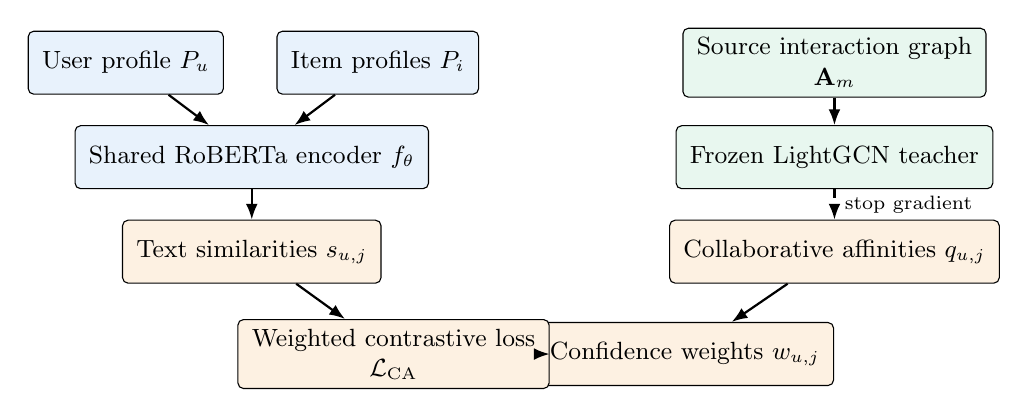
\begin{tikzpicture}[
    box/.style={draw, rounded corners=2pt, minimum height=8mm, align=center, font=\small, inner xsep=5pt},
    arrow/.style={-{Latex[length=2mm]}, thick},
    dashedarrow/.style={-{Latex[length=2mm]}, thick, dashed}
]
\node[box, fill=lightblue] (up) at (0,2.4) {User profile $P_u$};
\node[box, fill=lightblue] (ip) at (3.2,2.4) {Item profiles $P_i$};
\node[box, fill=lightgreen] (graph) at (9.0,2.4) {Source interaction graph\\$\mathbf{A}_m$};

\node[box, fill=lightblue] (encoder) at (1.6,1.2) {Shared RoBERTa encoder $f_\theta$};
\node[box, fill=lightgreen] (teacher) at (9.0,1.2) {Frozen LightGCN teacher};

\node[box, fill=lightorange] (sim) at (1.6,0) {Text similarities $s_{u,j}$};
\node[box, fill=lightorange] (aff) at (9.0,0) {Collaborative affinities $q_{u,j}$};
\node[box, fill=lightorange] (weight) at (7.1,-1.3) {Confidence weights $w_{u,j}$};
\node[box, fill=lightorange] (loss) at (3.4,-1.3) {Weighted contrastive loss\\$\mathcal{L}_{\mathrm{CA}}$};

\draw[arrow] (up) -- (encoder);
\draw[arrow] (ip) -- (encoder);
\draw[arrow] (encoder) -- (sim);
\draw[arrow] (graph) -- (teacher);
\draw[dashedarrow] (teacher) -- node[right,font=\scriptsize]{stop gradient} (aff);
\draw[arrow] (aff) -- (weight);
\draw[arrow] (sim) -- (loss);
\draw[arrow] (weight) -- (loss);
\end{tikzpicture}
\caption{Overview of \method. The trainable text path is identical to EasyRec. A source-domain LightGCN teacher is trained once and frozen; it affects only the weights of in-domain batch negatives. The green branch is removed during zero-shot inference.}
\label{fig:overview}
\end{figure*}

\subsection{Collaborative Confidence Teacher}

For every source domain $\mathcal{D}_m$, we train a standard LightGCN teacher on $\mathbf{A}_m$ with Bayesian personalized ranking.
LightGCN propagates embeddings over the bipartite graph without feature transformations or nonlinear activations \citep{he2020lightgcn}.
Let $\mathbf{g}_u$ and $\mathbf{g}_j$ be its final user and item embeddings.
The frozen teacher affinity is
\begin{equation}
q_{u,j}=\mathbf{g}_u^\top\mathbf{g}_j.
\end{equation}
The teacher is not treated as ground truth.
Instead, it provides relative evidence that an unobserved item is behaviorally compatible with the user.
Freezing the teacher prevents a degenerate solution in which it changes merely to reduce the text encoder's loss.

EasyRec mixes six Amazon source domains.
Teacher scores are meaningful only when $u$ and $j$ belong to the same interaction graph.
We therefore apply confidence weighting to same-domain negatives and assign $w_{u,j}=1$ to cross-domain negatives.
This rule also avoids inventing cross-domain identities or connections.

\subsection{Affinity Calibration and Weighting}

Raw inner products are not calibrated across users or domains.
For user $u$, we standardize the teacher scores of its same-domain batch negatives:
\begin{equation}
\hat q_{u,j}=
\sigma\left(\frac{q_{u,j}-\mu_u}{\sigma_u+\delta}\right),
\end{equation}
where $\mu_u$ and $\sigma_u$ are the mean and standard deviation over the available same-domain negatives, $\sigma(\cdot)$ is the logistic function, and $\delta$ ensures numerical stability.
The confidence-aware negative weight is
\begin{equation}
w_{u,j}=\epsilon+(1-\epsilon)(1-\hat q_{u,j})^\gamma,
\label{eq:weight}
\end{equation}
with floor $\epsilon\in(0,1]$ and sharpness $\gamma>0$.
A high teacher affinity produces a small weight, limiting the repulsive gradient on a possible false negative.
A low affinity produces a weight close to one.
The floor preserves some discrimination and protects against teacher mistakes.
If fewer than two same-domain negatives occur for a user, we use unit weights because batch calibration would be unstable.

\subsection{Confidence-Aware Objective}

We replace the denominator of Equation~\ref{eq:easyrec} with a weighted negative sum:
\begin{equation}
\begin{aligned}
Z_u^{\mathrm{CA}} &=
\exp(z_{u,i_u^+})+
\sum_{j\in\mathcal{N}_u^-}w_{u,j}\exp(z_{u,j}),\\
\mathcal{L}_{\mathrm{CA}}^{u\rightarrow i}
&=-\frac{1}{|\mathcal{B}|}\sum_{u\in\mathcal{B}}
\log\frac{\exp(z_{u,i_u^+})}{Z_u^{\mathrm{CA}}}.
\end{aligned}
\label{eq:caloss}
\end{equation}
The final objective is
\begin{equation}
\mathcal{L}=\mathcal{L}_{\mathrm{CA}}^{u\rightarrow i}
+\lambda\mathcal{L}_{\mathrm{MLM}}.
\end{equation}
All teacher-derived weights are detached from autograd.

This modification preserves the encoder, profile diversification, and cosine retrieval used by EasyRec.
During training, the $|\mathcal{B}|\times|\mathcal{B}|$ teacher affinities can be gathered from precomputed embeddings.
The additional operations are element-wise calibration and weighting over a similarity matrix that EasyRec already constructs.
At target-domain inference, only $f_\theta$ is retained, so latency and model size are unchanged.

\section{Experiments}

\subsection{Research Questions}

The experiments are designed around four questions.
\textbf{RQ1}: Does confidence-aware weighting improve zero-shot ranking over a reproduced EasyRec baseline?
\textbf{RQ2}: Are gains concentrated among sparse users, for whom unobserved feedback is most ambiguous?
\textbf{RQ3}: Does the teacher identify plausible false negatives rather than simply suppressing difficult examples?
\textbf{RQ4}: How sensitive is the method to $\epsilon$, $\gamma$, and the teacher choice?

\subsection{Datasets and Protocol}

We follow EasyRec's public split \citep{ren-huang-2025-easyrec}.
Six Amazon Review categories \citep{ni2019amazon} provide 124,732 source users, 67,455 source items, and 802,869 interactions for encoder training.
Zero-shot evaluation uses disjoint Sports, Steam, and Yelp data.
Their profiles and splits are provided by the EasyRec repository; no target interaction is used to update the text encoder.
Table~\ref{tab:data} reproduces the published statistics.

\begin{table}[t]
\centering
\small
\begin{tabular}{lrrr}
\toprule
Split / Domain & Users & Items & Interactions \\
\midrule
Train (6 domains) & 124,732 & 67,455 & 802,869 \\
\quad Arts & 14,470 & 8,537 & 96,328 \\
\quad Games & 17,397 & 8,330 & 120,255 \\
\quad Movies & 16,994 & 9,370 & 134,649 \\
\quad Home & 22,893 & 13,070 & 131,556 \\
\quad Electronics & 26,837 & 14,033 & 165,628 \\
\quad Tools & 26,141 & 14,155 & 154,453 \\
\midrule
Sports & 21,476 & 12,741 & 132,400 \\
Steam & 23,310 & 5,237 & 316,190 \\
Yelp & 11,091 & 11,010 & 166,620 \\
\bottomrule
\end{tabular}
\caption{Dataset statistics reported by \citet{ren-huang-2025-easyrec}. The first six domains train the encoder; the bottom three are used for zero-shot testing.}
\label{tab:data}
\end{table}

We use all-rank evaluation and report Recall@10/20 and NDCG@10/20.
Interacted items in the input history are masked before ranking.
The primary comparison uses EasyRec-Small (82M parameters) to make full retraining feasible; EasyRec-Base is an optional scale check.
All trainable variants use identical profiles, batches, seeds, and evaluation code.
We report mean and standard deviation over five runs and use paired two-sided tests at $p<0.05$.

\subsection{Baselines and Implementation}

The direct baseline is the released EasyRec objective.
We also include: (1) RoBERTa without collaborative tuning; (2) EasyRec with random weights sampled to match the mean of Equation~\ref{eq:weight}; (3) hard filtering, which discards the highest-affinity negatives; and (4) a popularity-based weight that does not use personalized teacher scores.
These controls distinguish useful personalized confidence from generic regularization.

We implement the method in PyTorch \citep{paszke2019pytorch} on the public EasyRec code.
Following the original setup, $\tau=0.05$, $\lambda=0.1$, the MLM masking ratio is 0.15, the learning rate is $5\times10^{-5}$, and training lasts 25 epochs.
LightGCN teachers use the same source training edges and are selected on source validation Recall@20.
The initial grid is $\epsilon\in\{0.1,0.3,0.5,0.7\}$ and $\gamma\in\{0.5,1,2\}$.
Hyperparameters are selected only on source validation data.

\subsection{Main Results Template}

Table~\ref{tab:main} separates numbers reported in the EasyRec paper from results that must be generated locally.
The reported row is a reference point, not evidence that our environment reproduces the baseline.
The main claim will be supported only if \method{} improves the reproduced EasyRec row consistently, rather than merely approaching a published checkpoint.

\begin{table}[t]
\centering
\small
\begin{tabular}{llcc}
\toprule
Dataset & Method & R@20 & N@20 \\
\midrule
\multirow{3}{*}{Sports}
& EasyRec-S (reported) & .0286 & .0135 \\
& EasyRec-S (reproduced) & \pending & \pending \\
& \method{} & \pending & \pending \\
\midrule
\multirow{3}{*}{Steam}
& EasyRec-S (reported) & .0174 & .0097 \\
& EasyRec-S (reproduced) & \pending & \pending \\
& \method{} & \pending & \pending \\
\midrule
\multirow{3}{*}{Yelp}
& EasyRec-S (reported) & .0046 & .0026 \\
& EasyRec-S (reproduced) & \pending & \pending \\
& \method{} & \pending & \pending \\
\bottomrule
\end{tabular}
\caption{Zero-shot recommendation template. ``Reported'' values are copied from \citet{ren-huang-2025-easyrec}; all \pending{} cells require actual runs. Final tables will include standard deviations and significance marks.}
\label{tab:main}
\end{table}

\subsection{Diagnostic and Ablation Plan}

Accuracy alone cannot verify the proposed mechanism.
We therefore conduct a \emph{masked-positive audit}: for source users with at least two interactions, one observed item is temporarily hidden and mixed with 99 unobserved items.
The frozen teacher must rank the held-out positive highly if its confidence is informative.
We report teacher AUC and Recall@10, together with the proportion of training negatives assigned $w_{u,j}<0.5$.
This exposes a failure mode in which the teacher merely assigns uniformly low weights.

For sparsity analysis, target users are divided by history length into $[1,5]$, $[6,10]$, and $[11,\infty)$ groups.
The hypothesis is that confidence-aware source training benefits the first group most, but this statement will be accepted only after the stratified results are observed.
Table~\ref{tab:ablation} isolates each design decision.

\begin{table}[t]
\centering
\small
\begin{tabular}{lccc}
\toprule
Variant & Sports & Steam & Yelp \\
\midrule
EasyRec-S & \pending & \pending & \pending \\
\method{} & \pending & \pending & \pending \\
\quad w/o teacher (random) & \pending & \pending & \pending \\
\quad hard filtering & \pending & \pending & \pending \\
\quad popularity weight & \pending & \pending & \pending \\
\quad no weight floor ($\epsilon=0$) & \pending & \pending & \pending \\
\quad in-domain-only batches & \pending & \pending & \pending \\
\bottomrule
\end{tabular}
\caption{Ablation template using Recall@20. Every entry is pending execution.}
\label{tab:ablation}
\end{table}

Sensitivity curves vary $\epsilon$ and $\gamma$ while holding all other settings fixed.
We additionally record training time and target inference latency.
Because the teacher is removed after training, target inference should match EasyRec within measurement noise; this is a system expectation to be checked, not a reported result.

\subsection{Decision Rule}

We will regard the modification as supported when it improves the average of Recall@20 and NDCG@20 over the reproduced EasyRec baseline across the three targets, does not cause a relative degradation larger than 1\% on any target, and shows its largest or second-largest gain in the sparse-user group.
If ranking improves but the teacher fails the masked-positive audit, the mechanism claim will be rejected and the effect interpreted as generic reweighting.
If random weighting matches \method, the collaborative teacher is unnecessary.
These criteria prevent a post-hoc explanation based only on favorable aggregate numbers.

\section{Conclusion}

We introduced \method, a focused extension of EasyRec for positive-unlabeled recommendation data.
The method uses frozen source-domain LightGCN teachers to estimate which in-batch negatives may be compatible with a user's collaborative preference.
It then down-weights those pairs in EasyRec's contrastive denominator while leaving reliable negatives, the textual encoder, and zero-shot inference intact.
The proposal is deliberately small: it addresses one identifiable assumption, requires no target graph at deployment, and supports direct ablation against the public baseline.
This draft provides the complete method and evaluation protocol but makes no empirical superiority claim before the experiments are run.
The next step is to reproduce EasyRec-Small under the released setup, implement Equation~\ref{eq:caloss}, and fill the marked tables with five-run results.

\section*{Limitations}

LightGCN scores are estimates learned from the same sparse graph and can inherit popularity or exposure bias.
The weight floor reduces but does not eliminate this risk.
Teacher training adds source-side computation, and maintaining one teacher per domain may be inconvenient when the number of domains is large.
The current method handles only implicit feedback and English textual profiles.
Finally, the proposed confidence rule is evaluated through offline ranking; online user satisfaction cannot be inferred from Recall or NDCG alone.

\section*{Ethical Considerations}

Personalized profiles may encode sensitive preferences or amplify historical exposure patterns.
Experiments should use the anonymized public data distributed with EasyRec and should not attempt to re-identify users.
Generated profiles must be inspected for unsupported demographic attributes.
Confidence weighting should not be interpreted as proof that a user likes an item, and deployment would require fairness, privacy, and feedback-loop monitoring beyond this course project.

\bibliography{references}

\end{document}
